\subsection{Proportional controller test} %\label{put a label here and uncomment}
\textbf{Name: Group 510}\\
\textbf{Date: 06/10 - 2015}

\subsubsection{Purpose}
The purpose of this test is to find out how the system reacts to closed loop control.
\\

\subsubsection{Theory}
According to \todo{source}, a P-controller makes it possible to change the time constant of a system. To test this, a P-controller with a gain of 1 is implemented, and compared to a normal step response.
A side effect of the Proportional control is a steady state offset. This can be easily shown by an example:

A non moving system, with a desired final speed of 2 m/s, and a P-gain of 1 is examined.

In the beginning, the error will be calculated as $$\SI{2}{m/s} - \SI{0}{m/s} = \SI{2}{m/s}$$
The system is therefore instructed to accelerate to 2 m/s.

After a period of time, the system will cross 1 m/s. Calculating the error now, results in $$\SI{2}{m/s}-\SI{1}{m/s}=\SI{1}{m/s}$$
The system is therefore instructed to stay at 1 m/s, and stop accelerating. This effectively causes a steady state error of 50\%.

A way to reduce this offset is to use Feed Forward. \todo{source}. This will be tested as well, with a Feed Forward gain of 1.



\subsubsection{Setup}

\begin{figure}[H]
	\centering
	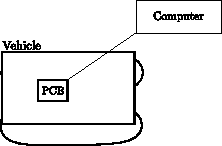
\includegraphics[scale=1.6]{figures/inertiaTestSetupDiagram2.pdf}
	\caption{Setup diagram}
	\label{GainAndTimeTestSetupDiagram}
\end{figure}

\subsubsection{List of Equipment}

\begin{table}[H]
\begin{tabular}{|p{10cm}|p{4cm}|}
\hline%------------------------------------------------------------------------------------
  \textbf{Instrument}                     &  \textbf{Type}       \\
\hline%------------------------------------------------------------------------------------
  Computer                                &  HP 8460P    \\
\hline %-----------------------------------------------------------------------------------
\end{tabular}
\end{table}

\subsubsection{Procedure}

\begin{enumerate}
  \item Disconnect the battery.
  \item Connect the Arduino to the computer.
  \item Upload the test code to the Arduino board using the Arduino IDE  \cite{ArduinoIDE}.
  \item Open a serial terminal via PuTTY \cite{PuTTY}.
  \item Plug in the battery immediately after opening the terminal.
  \item Wait two seconds, then follow the vehicle with the connected computer.
  \item Wait until the vehicle stops before ending the measurements by unplugging the connected computer from the Arduino.
  \item Plot the speed of the vehicle using Matlab.
\end{enumerate}
\subsubsection{Results}
\begin{figure}[H]
  \centering
 	%Trim margins @:   left        bottom       right       top
 	\adjustbox{ trim = {.15\width} {.30\height} {.15\width} {.30\height}, clip }
  {
    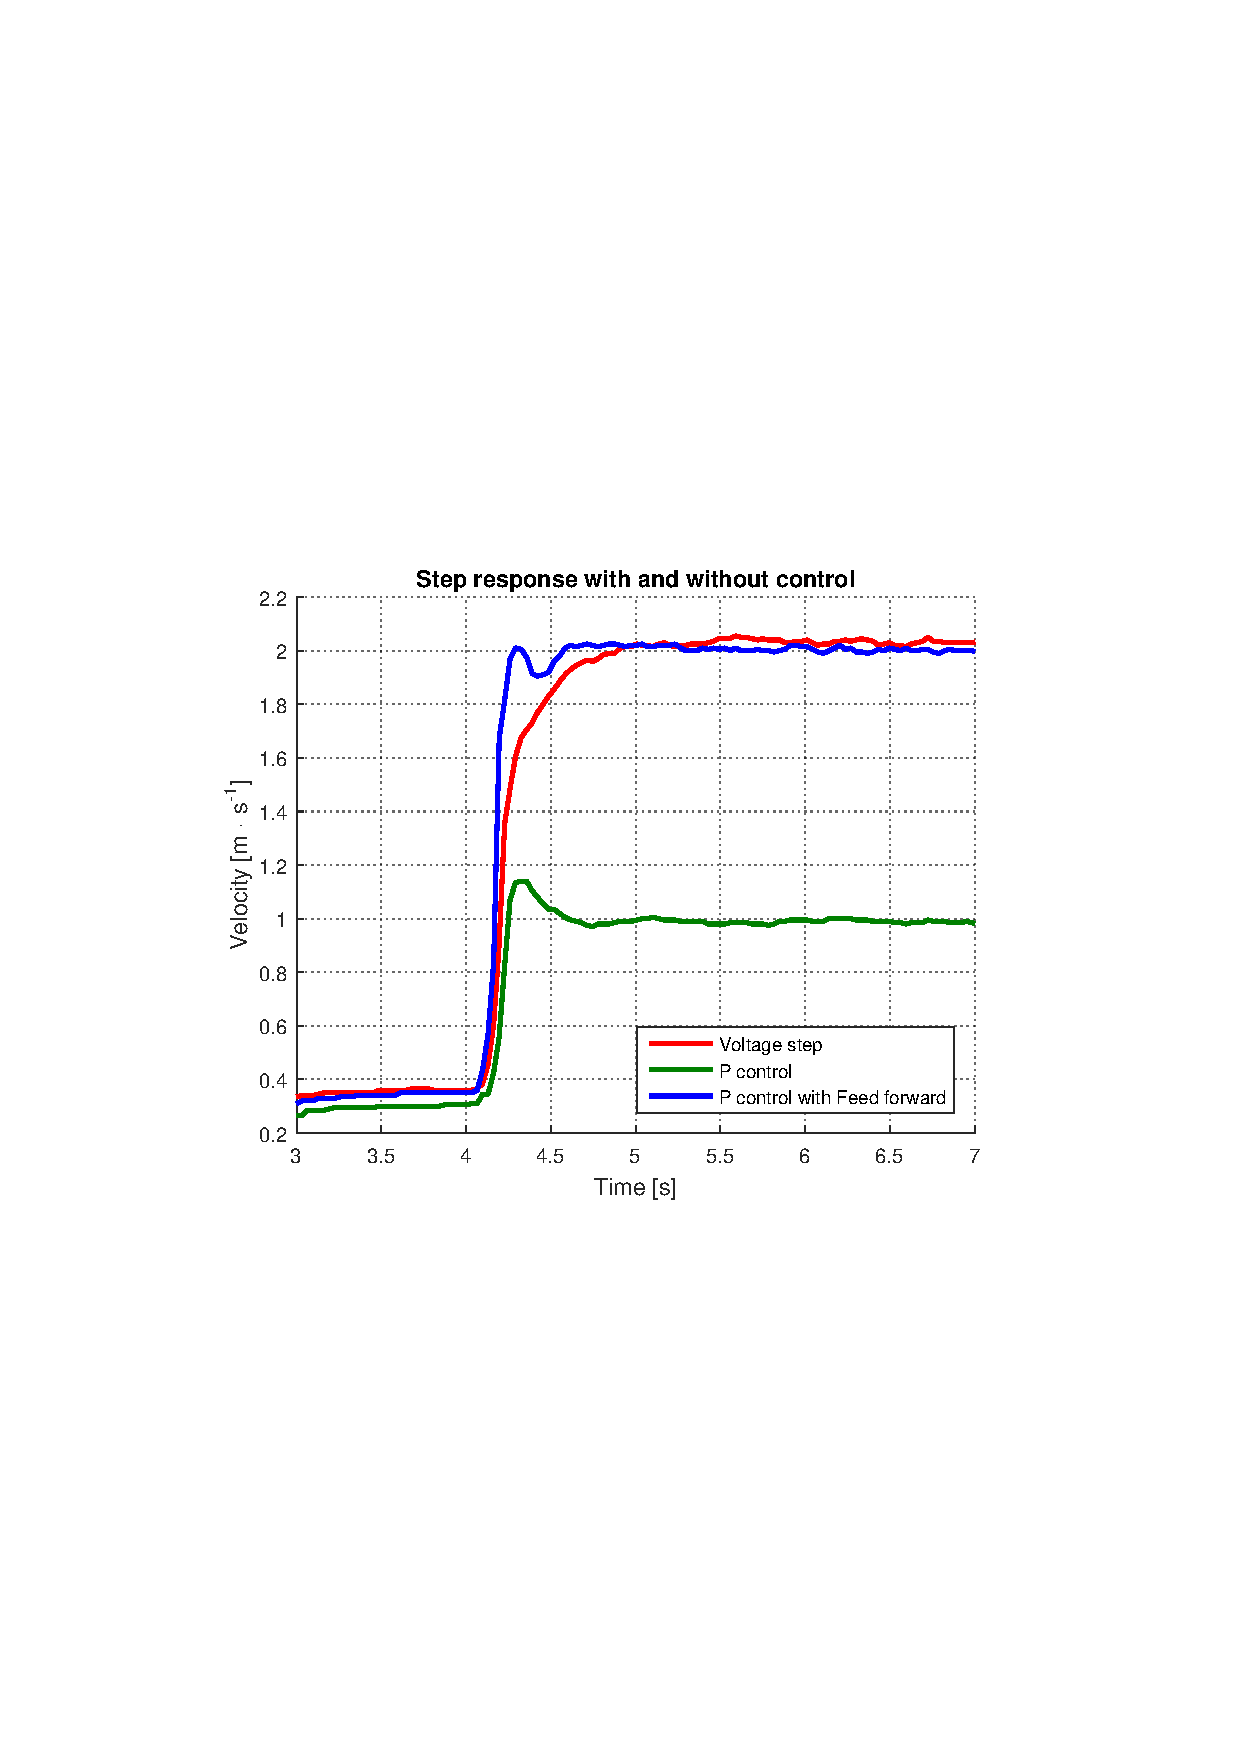
\includegraphics[width=1.4\textwidth]{figures/stepWithPControl.pdf}
  }
  \caption{A plot illustrating the step responses with and without P control}
  \label{PconTest}
\end{figure}

In all tests, the vehicle was instructed to change its speed from $\SI{0,3}{m/s}$ to $\SI{2}{m/s}$.
The resulting responses of the system can be seen in \figref{PconTest}. It can be clearly seen, that the P-controller creates an offset of 50\%, just as expected. The Feed forward eliminates this error. The three time constants can now be reviewed:
$$\tau_\text{s}=\SI{0,211}{s}$$
$$\tau_\text{p}=\SI{0,152}{s}$$
$$\tau_\text{f}=\SI{0,152}{s}$$
\hspace{6mm} Where:\\
\begin{tabular}{p{1cm}lll}
& $\tau_\text{s}$ & is the time constant for the open loop response &\unitWh{s}\\
& $\tau_\text{p}$       &is the time constant for the response with a P-controller&\unitWh{s}\\
& $\tau_\text{f}$   & is the time constant for the response with a P-controller and feed forward&\unitWh{s}\\
\end{tabular}

It can be concluded, that the P controller lowers the time constant of the system. Furthermore it is clear, that the feed forward does not affect the time constant, just the final speed.